\documentclass{article}
\usepackage{graphicx} % Required for inserting images
\usepackage[backend=biber, style=numeric]{biblatex}
\usepackage{float}
\usepackage{booktabs}
\usepackage{appendix}
\usepackage{amsfonts}
\usepackage{tabularx}
\usepackage{amsmath}
\usepackage{hyperref}
\newcolumntype{W}[1]{>{\hsize=#1\hsize\raggedright\arraybackslash}X}
\addbibresource{references.bib}
\AddToHook{cmd/section/before}{\clearpage}
\title{An Exploration of Machine Learning for zero-day detection in network Intrusion Detection Systems}
\author{Omar Hyder}
\date{July 2026}

\begin{document}
\maketitle
\begin{abstract}
    Machine-learning intrusion detection systems routinely report $>99\%$ accuracy, but on random splits that expose every attack type during training. This write-up seeks to investigate what happens when models are introduced to zero-days. I conducted two experiments on the CIC-IDS2017 dataset: a random split and an unseen-class split, comparing XGBoost, Isolation Forest and Local Outlier Factor models. With all attack classes seen, XGBoost reaches a false-positive rate $\sim$1-2\% and a macro attack recall $\sim$0.85. With none seen, macro attack recall falls to 0.23 and weighted recall to 0.01. Unsupervised anomaly detectors recover 0.67-0.76 macro attack recall at the cost of 37-46\% FPR. Their relative ranking reverses between validation and test depending on which unseen attack are present, suggesting even zero-day focused evaluation can mislead. I intend to display the gap between known-attack and zero-day performance, expose how it is architecture agnostic, and advocate for held-out class splits to be a standard in future machine-learning intrusion detection systems research. 
	\par \href{https://github.com/OmarHyder07/ML-IDS}{Notebooks available on GitHub.}
\end{abstract}

\tableofcontents

\section{Introduction}
Intrusion Detection Systems (IDS) are integral to network security, acting as a first layer of defense by flagging malicious traffic. Recent LLM developments have raised concerns about automated exploitations of zero-day attacks. Yet, developments in ML also lead to developments in IDS technology beyond traditional methods such as firewalls and access control mechanisms\parencite{Hozouri2025}.
\subsection{Current State of ML-IDS Research}
Many highly optimized systems, such as the ensemble-based NIDS proposed by Patil et al. (2025)\parencite{Patil2025}, achieve near-perfect metrics (e.g., 99.98\% accuracy) on the CIC-IDS2017 dataset using standard randomly stratified 70/30 splits. Moczkodan and Ragab (2026)\parencite{moczkodan2026} propose the use of temporal architectures such as Transformers. They too used CIC-IDS2017 on a random split. The aforementioned dataset is split into 8 CSVs across 5 simulated days. Each day contains "flow" data \textit{(see appendix for notes on networking terminology)} with unique attack types, for example, only Thursday contains web attacks such as SQL injection and cross-site scripting, while only Friday contains DDoS flows. The key issue being, as they test on the exact same days and attack types they trained on, these metrics do not reflect chronological generalisability or vulnerability to zero-day events. In fact, in the Realistic Evaluation section of Moczkodan and Ragab's paper, they evaluate their model and 8 other ML and DL architectures under a time-based split (unseen attacks in test set), finding macro-F1 collapsed to $\sim$50\% for all models - not nearly suitable for a deployment-ready IDS. While many papers in the field use highly sophisticated, bleeding-edge architectural designs, I believe the use of a random split greatly detracts from some of the achieved near-perfect evaluation metrics. In this write-up I propose and attempt to justify that modern IDS research should reflect our uncertain and volatile modern technological landscape by placing greater emphasis on zero-day detection.
\section{CIC-IDS2017}
This report is an exploration of this technology using the CIC-IDS2017 dataset. This dataset was generated using a network environment with various clients, using open-source tooling designed to simulate both benign and malicious traffic\parencite{sharafaldin2018}. It is a modern, flow-based, realistic dataset. I previously worked on supervised methods on the NSL-KDD dataset, which is much older (2009) and simpler, providing less realistic model evaluation. Engelen et al. discuss the limitations in validity and overall utility of the dataset at depth\parencite{engelen2021troubleshooting}. They also offer relevant fixes, and released an improved version of the dataset. While I will attempt to follow their warnings as closely as possible, I will choose to keep the dataset as I want any negative results to hold on a version which the field actually reports on.
\subsection{Data \& Pre-processing}
There are $\sim$2.8M flows from 8 CSV files, spread across a simulated working week, Mon-Fri, with $\sim$80 features and 15 distinct classes (flow data extracted from packet captures). 
\par Pre-processing is handled in the following steps:
\begin{enumerate}
  \item All 8 CSVs are joined into one set,
  \item Column names are stripped of leading whitespace and non-UTF8 characters are normalised,
  \item \textbf{inf} values are replaced with \textbf{NaN},
  \item Rows with \textbf{NaN} values are dropped (2,867 rows). Notably, this does not remove examples from any ultra-rare classes,
  \item Columns are downcast from \textit{float64} to \textit{float32} where relative error $< 1e-07$.
\end{enumerate}
De-duplication also occurs, however I will be trialling different splits of the data which require different considerations. The above are common steps to each section of investigation. 

\section{Supervised performance under a random split}
This section aims to reproduce high evaluation-metrics on a random stratified split of data. I explore different methods of improving the XGBoost ensemble's performance through the use of various imbalance-handling techniques. 
\paragraph{Setup} A controlled comparison of imbalance handling techniques: identical model and hyper-parameters throughout (XGBoost, 300 estimators, learning rate 0.1, 20 early-stopping rounds, ‘hist‘ tree method, fixed random state), identical held-out test set, resampling fit on training data only. Notably, I am joining each "days" data into one large set. I then de-duplicated rows (dropping 307,084) to avoid leakage across sets. Train, test and cross validation receive a random stratified sample (60/20/20). Only the imbalance-handling method varies. \href{https://github.com/OmarHyder07/ML-IDS/tree/main/cic-ids2017}{\textit{See notebook for methodology.}}
\paragraph{Features and Leakage}
Permutation importance measures how test performance drops when a feature's values are shuffled. This is a trustworthy signal as it captures non-linear relationships between features and classes. It can \textit{under-report} a feature when a collinear partner covers for it, as XGBoost will split on one and leave the other apparently unimportant simply based on which it got to first. This is a limitation. Low-ranked features that are strongly correlated with high-ranked features won't be listed. So, I won't analyse features individually but rather as buckets / classes of features. The following permutation importance results are of a "baseline" XGBoost model trained with the aforementioned hyper-parameters and no imbalance handling.
\begin{itemize}
        \item \#1 Destination Port 
        \item Connection setup fingerprints - \#2 Init\_Win\_bytes\_forward and \#5 backwards. Attack tools often use non-standard stacks that differentiate them from normal traffic.
        \item Traffic volume and shape - \#3 Total Length of Fwd Packets, \#4 Fwd Header length. Also highly rated: Packet Length Mean, Fwd/Bwd Packet Length Max/Std, Average Packet Size, Bwd Header Length. These show how much data flowed and how it was distributed. Floods, scans and brute-force attacks each have characteristic volume signatures which the model picked up on.
          
        \item Timing - \#6 Fwd IAT Min, also Flow IAT Min, Fwd IAT Std, Flow Packets/s. Gaps between packets and packet rate. Tool-generated attacks have unnaturally regular or extreme timing.
\end{itemize}
\subsection{Shortcut learning?} CICIDS-2017 was generated in a controlled lab with attacks run against a specific service on their standard port. FTP-Patator against 21, SSH-Patator against 22. Web attacks against 80. Thus, the destination port feature acts almost as a direct label for some attack classes. A model can "detect" FTP-Patator by just learning the mapping of port 21 to the attack type. This is known as \textit{shortcut learning}, and prevents the model from learning the true pattern of the attacks, causing issues in actual deployment. Attacks can target non-standard ports so a model trained with the destination port feature will not be reliable in deployment! Engelen et al. discuss the methodology used to create synthetic traffic in the dataset: "... in all cases
these features do not have any semantic connection with the
intended malicious activity, but rather stem from the specifics
of the used attack tools."\parencite{engelen2021troubleshooting}
\par The offending features they list are: Destination Port, Init\_Win\_bytes\_forward, Fwd Header Len, Total Fwd Pkt, Min Seg Size Fwd, and the flow-separators SYN Flag Count and Bwd Pkt Len Mean. This is corroborated by my permutation importance analysis. The most important feature buckets could all be evaluated as quirks of an attack generating tool. 

\begin{table}[H]
\centering
\makebox[\textwidth][c]{%
\begin{tabular}{@{}llrccc@{}}
\toprule
\textbf{Freq.} & \textbf{Classes} & \textbf{n} & \textbf{Recall} & \textbf{Recall} & \textbf{$\Delta$} \\
               \textbf{band}     &                  &       \textbf{(test)}            & \textbf{(all feat.)} & \textbf{(no shortcuts)} & \\
\midrule
 --- & Benign & 418,794& $\sim$1.00& $\sim$1.00& $\approx$0.00\\
$>$10{,}000 & DDoS, PortScan, DoS Hulk            & 78,599& $\sim$1.00& $\sim$1.00& $\approx$0.00\\
$>$1{,}000  & DoS GoldenEye/Slowhttptest/slowloris, FTP-Patator & 5,298& $\sim$1.00& $\sim$0.99& $-$0.01\\
$>$100      & Web Brute Force, Web XSS, Bot, SSH-Patator  & 1,452& $\sim$0.72& $\sim$0.63& $-$0.09\\
$>$0        & Heartbleed, Infiltration, Web SQL Injection & 15& $\sim$0.60& $\sim$0.53& $-$0.07\\
\midrule
\multicolumn{3}{@{}l}{\textit{Macro-avg recall}}          & 0.86& 0.83& $-$0.03\\
\multicolumn{3}{@{}l}{\textit{Macro-avg precision}}       & 0.90& 0.94& $+$0.04\\
\bottomrule
\end{tabular}}
\caption{Per-frequency-band recall with and without the shortcut-learning
features (Destination Port, Init\_Win\_bytes\_fwd, Fwd Header Len, Total Fwd Pkt,
Min Seg Size Fwd, SYN Flag Count, Bwd Pkt Len Mean). }
\end{table}

\subsection{True baseline} I will find a true baseline from a feature set disregarding the above. All future models will be trained on this feature set.


The effect concentrated almost entirely on the Bot class (n=403), whose recall fell from 78\% to 45\%; possibly the only class materially dependent on the shortcut features. SSH-Patator (n=639) fell marginally, 100\% to 95\%. Higher-frequency classes were unaffected, suggesting that sufficient data lets the model learn genuine attack patterns instead of tool fingerprints.
\par Generally, recall steeply declines with low-frequency classes. Should I spend time tweaking and tuning XGBoost hyper-params? Not quite. This is indicative of an \textit{imbalance} issue, not model failure.


\subsection{Imbalance Experiment}
\paragraph{Method}
There are many methods for dealing with imbalance. I will conduct a fair test to trial some of these methods in isolation. Each test will use the same XGBoost model with the same hyper-parameters. The meaningful metrics are per-attack-class recall, but since there are 14 attack classes I will report \textbf{macro-averaged} recall and precision. With such imbalanced datasets, per-class recall is also a very important metric, which will be discussed where interesting. 
\begin{figure}[H]
\makebox[\textwidth][c]{%
    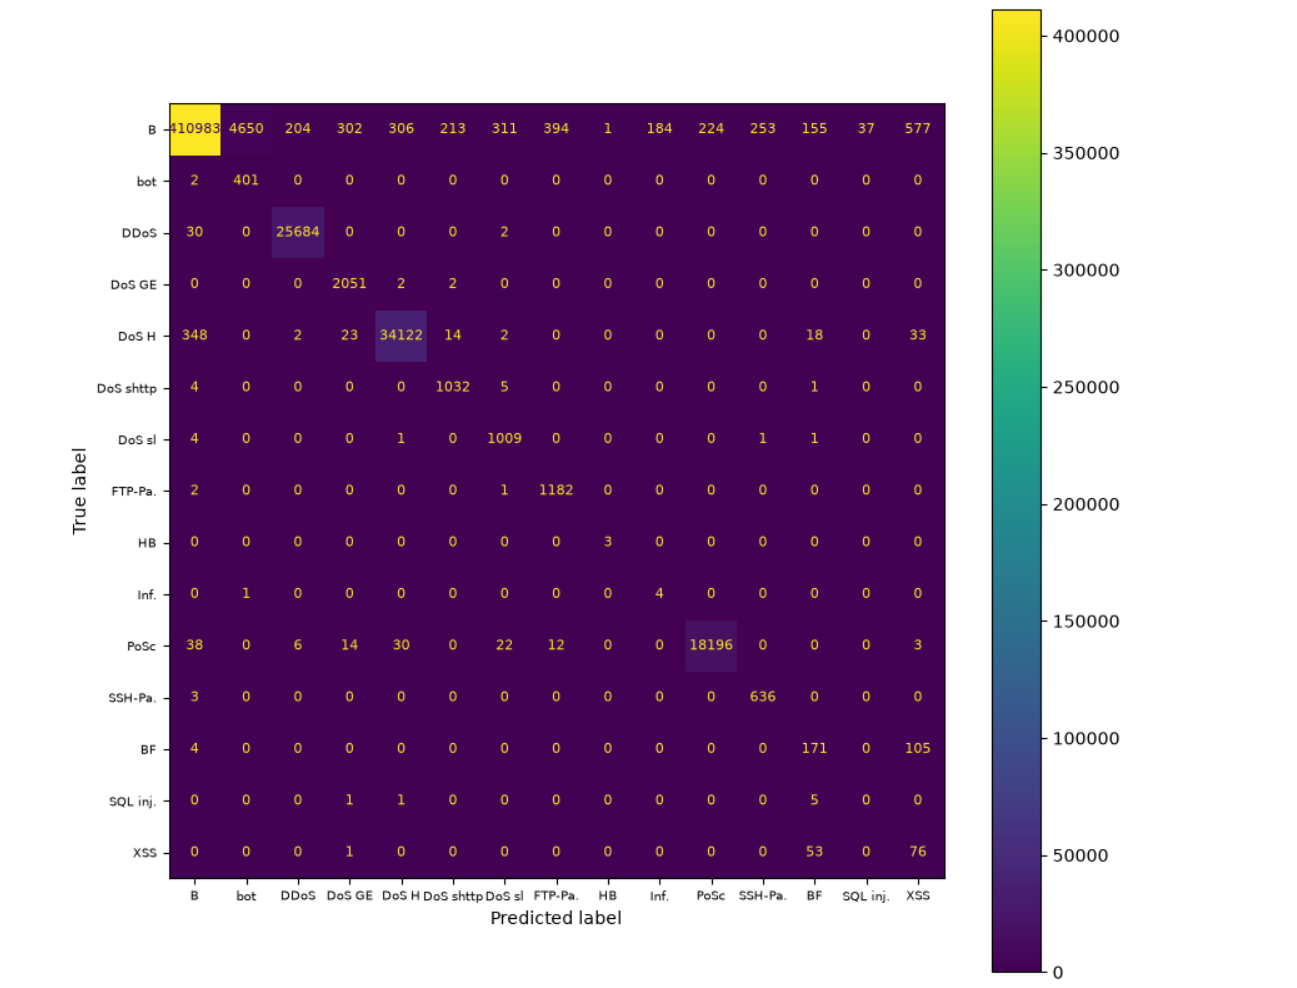
\includegraphics[width=1.5\textwidth]{Screenshot From 2026-08-26 15-33-18.png}
}
    \caption{Confusion matrix of U-O-U synthesis model}

\end{figure}
\begin{table}[H]
\centering
\makebox[\textwidth][c]{%
\begin{tabular}{@{}ll|llll@{}}
\toprule
\textbf{Type} & \textbf{Technique} & \textbf{FPR} & \textbf{Alert} & \textbf{Macro attack} &  \textbf{Weighted attack} \\
              &                    &               & \textbf{precision} & \textbf{recall} & \textbf{recall}  \\
\midrule
Baseline & ---                            & $\sim$0.00 & 0.99& 0.82 & 0.99\\
Weights  & Sample weights                 & 0.01 & 0.93& 0.86 & $\sim$1.00\\
Under    & Cluster-centroid               & 0.05& 0.81& 0.86& $\sim$1.00\\
Under    & Random $\to$ ENN               & 0.04 & 0.82 & 0.81& 0.99\\
Over     & Naive random oversampling      & $\sim$0.00 & 0.99& 0.82& 0.99\\
Over     & SMOTE                          & $\sim$0.00 & 0.99& 0.83& 0.99\\
U-O-U& Random $\to$ SMOTE $\to$ ENN & 0.02 & 0.91& 0.86& 0.99\\
\bottomrule
\end{tabular}}
\caption{Imbalance techniques: Baseline (none) vs. Sample Weights vs. Under-Sampling vs. Over-Sampling vs. Over-Under synthesis, with XGBoost, common hyper-parameters, same train and test set, resampling fit on train only.} 
\end{table}
False positive rate is a very insightful first metric. A real SOC team would be overwhelmed at anything above $\sim$5\% FPR; constant false-alarms would cost a huge amount of time and money. Over-sampling techniques left FPR near baseline, under-sampling cost 4\%. Sample weights is thus a clear winner, it has the best trade off of high recall (0.87) without increasing the FPR too high (1.43). Despite this, for further analysis I will focus on the synthesis of U-O-U. Under-sampling methods drastically reduce training time, and the synthesis brought this with only a modest increase to FPR from the sample weights method. This is highly practical: if retraining with new, real-world network traffic, speed and minimal compute use will be highly important. Oversampling also has the most interesting failure mode for dissection.
\par From analysing the confusion matrix of the imbalance technique synthesis model (Figure 1), we see the majority of errors arise from false-positives, where benign flows are misclassified as anomalous. This is most striking with the "Bot" class, with 4650 benign flows classified as Bot. This is unsurprising. A botnet tool creates seemingly benign pings to a central command server, which are unnaturally regular. This leads to a "flaw" with oversampling - the model will over-predict rare classes. Here, it will be more sensitive towards the botnet fingerprint, so much so that it assigns many benign flows to the Bot class. Thus, recall for the bot class is near perfect, while precision is 0.08. The baseline had recall of the bot class at 0.45. The synthesis brought perfect recall at the cost of 4,650 false alarms. However, since the false positive rate is generally so low, perhaps a security team would take this trade-off. Missing an attack could have catastrophic consequences, however all of the Bot attack flows occur over one simulated Friday. A security team would have to evaluate if they have enough resources to deal with 4,650 false alarms in one day so as to prevent missing any malicious flows.
\par SQL Injection is particularly bad, with every example misclassified. This is also unsurprising. Web attacks occur from malicious data within the \textit{payload} of packets. Since CIC-IDS2017 contains statistics about flows (such as payload size), without any of the actual data within the payload, SQL injection, cross-site scripting (XSS) will be difficult to differentiate from something like a brute force attack. How can we tell if data entered to a form is a password attempt or SQL queries if we have no access to the data itself? On the other hand, can imbalance handling techniques overcome extreme scarcity? With SQL Injection having only 9 examples in training, oversampling methods simply would not have enough variety of data to infer on. 
\par The only low-frequency class which stayed at zero recall is SQL Injection, which is payload-invisible, and the two mid-frequency web classes (BF n=280, XSS n=130) sit at $\sim$0.6 while similarly sized non-web classes are near 1.0. Heartbleed (3 test examples) got 3/3, Infiltration 4/5. Thus, we could say within this dataset extreme scarcity was not a bottleneck, but rather feature visibility.  Here, I failed on attack types with limited information. Perhaps a more sophisticated architecture would be able to pinpoint smaller fingerprints within the web attacks.
\begin{table}[]
\centering
\makebox[\textwidth][c]{%
\begin{tabular}{@{}llrccc@{}}
\toprule
\textbf{Freq.} & \textbf{Classes} & \textbf{n} & \textbf{Recall} & \textbf{Recall} & \textbf{$\Delta$} \\
               \textbf{band}     &                  &       \textbf{(test)}            & \textbf{(baseline)}& \textbf{(synthesis)}& \\
\midrule
 --- & Benign & 418,794& $\sim$1.00& $\sim$0.98& $-$0.02\\
$>$10{,}000 & DDoS, PortScan, DoS Hulk            & 78,599& $\sim$1.00& $\sim$0.99& $-$0.01\\
$>$1{,}000  & DoS GoldenEye/Slowhttptest/slowloris, FTP-Patator & 5,298& $\sim$0.99& $\sim$0.99& $\approx$0.00\\
$>$100      & Web Brute Force, Web XSS, Bot, SSH-Patator  & 1,452& $\sim$0.63& $\sim$0.79& $+$0.13\\
$>$0        & Heartbleed, Infiltration, Web SQL Injection & 15& $\sim$0.53& $\sim$0.65& $+$0.12\\
\midrule
\multicolumn{3}{@{}l}{\textit{Macro-avg recall}}          & 0.83& 0.87& $+$0.04\\
\multicolumn{3}{@{}l}{\textit{Macro-avg precision}}       & 0.94& 0.61& $-$0.33\\
\bottomrule
\end{tabular}}
\caption{Per-frequency-band recall comparison of baseline and with synthesis of imbalance handling techniques applied.}
\end{table}
\subsection{Verdict}  
While imbalance handling techniques created marked improvements in anomaly detection without raising the false-positive rate too high, the aforementioned results show nothing of the model's capacity to classify unseen attacks. Thus, a relevant direction of investigation would be to evaluate the same model on a split in which the test set contains unseen attack types.
\section{Unsupervised performance on a temporal split}
The following section justifies the use of, and explores the performance of various unsupervised algorithms applied to a day-by-day temporal split of data. Note that I am using the term "temporal" to mean time-based splitting, which in this context really can be defined as having unseen classes in the test set. The specific elements of delay, time or day of the week are irrelevant. 
\subsection{Day-by-day evaluation}
The previous split; joining all data together into one large set, then randomly splitting for train and test, allows the models to see every attack type in training. In real deployment, we won't be able to train the model on the attacks that appear in the future. 
\paragraph{Setup} Training on Monday-Wednesday, testing on Thursday-Friday. Of the 7 attack types present in the test set (Bot, DDos, PortScan, Infiltration, all Web Attacks: XSS, Sql Injection, BruteForce), all are unseen in the training set. In line with the previous section, I will first evaluate an XGBoost model under this split. Same hyper-parameters, same removal of shortcut learning features. Previously I de-duplicated on the entire set, as randomly sampling for train and test could create repeat instances of identical traffic in both sets, causing leakage. Here, duplicate rows between the temporal split are fine, as we are using a genuine rather than an artificial split. Thus, it will be skipped. As there are unseen categories, I will transform the classification from multiclass to binary - benign vs. anomalous.
\begin{table}[]
\centering
\makebox[\textwidth][c]{%
\begin{tabular}{@{}l|rr|rrrrrrr@{}}
\toprule
& \textbf{benign}& \textbf{anomaly}& \textbf{Bot}& \textbf{Infil.}&  \textbf{PortScan}& \textbf{DDoS}& \textbf{Sql Inj.}& \textbf{Brute Force}& \textbf{XSS} \\
\midrule
\textbf{n (test)} & 870,343 & 291,001 & 1,956 & 36 & 158,804 & 128,025 & 21 & 1,507 & 652 \\
\midrule
\textbf{Recall}& 0.99& 0.01& $\sim$0.00& $\sim$0.00& $\sim$0.00& $\sim$0.00& 0.33& 0.60&0.69\\
\bottomrule
\end{tabular}}
\caption{Supervised model (XGBoost) performance under a temporal-split of data. Recall split by class post-inference, as inference was binary-classification (benign vs. anomalous).}
\end{table}
\paragraph{Results} Steep drop in anomaly recall. From macro-average attack recalls of 0.82-0.87 on the random split to a macro attack recall of 0.23; with weighted attack recall, a drop from 0.99$\to$0.01. NSL-KDD had a drop of 0.71$\to$0.38 when introduced to unseen types. Here, under a harsher temporal split, it completely collapsed, reaffirming zero-days as the fundamental ceiling on supervised algorithms. The modicum of success on web attacks may be an artifact of resemblance to Wednesday's DoS attacks. 
\subsection{Anomaly Detection}
Supervised models structurally can not recognise what they have never seen. An approach that models \textit{normal} and flags deviation doesn't depend on having seen attacks, thus it fits as the next step of investigation for ML as an IDS.
\par I will be evaluating two methods: Isolation Forest and Local Outlier Factor, both trained on entirely benign flows. They have different mechanisms of anomaly detection, thus it will be of interest to compare the per-class performance of each.
\begin{itemize}
\item \textbf{iForest} finds points which can be separated with random cuts, i.e. globally sparse outliers and weird one-offs. For example, the PortScan class (in test), with its 1000s of near-identical flows, is likely to evade an iForest's detection. Whereas, infiltration, Heartbleed (in CV) and possibly the web attacks are more likely to be flagged due to their global uniqueness. 
\item \textbf{LOF} uses a density-based method with a different inductive bias. Due to the presence of unseen categories in the test set, along with training on benign only, I am training with novelty. This allows the LOF model to point out \textit{locally unique} examples, i.e. attacks which seem benign - ones which an iForest would miss. I predict it will excel on  brute force (Patator) (in CV), PortScan and DDoS.
\end{itemize}
\paragraph{Method} For both models, I will do one sweep of the \textit{contamination} parameter, and choose a value based on a precision-recall tradeoff. Specifically, choosing for highest recall where precision is at least 0.40. Contamination tells the model the proportion of anomalous examples present in the test / deployment data. The sweep will be conducted on a cross-validation set taken from the training days, thus avoiding leakage. Attack proportions are unpredictable however, volume varies by day and different attack types may have shallower or heavier traffic. Yet, this is a very real, deployment-esque limitation that should not be avoided. All of the attacks in Mon-Wed are concentrated in the cross-validation set, so the contamination proportion found may be artificially high, at least relative to test.
\begin{itemize}
\item Isolation Forest is an ensemble method which requires minimal hyper-parameter tuning. It also requires, if not benefits, from no data scaling.
\item Local Outlier Factor does require scaling. I will apply Robust Scaling to every numerical column, fit on the training set. Robust scaling uses median and inter quartile range to replace mean and standard deviation in z-scaling, making it more robust to extreme points. Due to LOFs quadratic time complexity, I will take a sub-sample of 200,000 benign examples from training. I will then do a single sweep of the number of neighbours parameter.
\end{itemize}
Both trained entirely on benign examples from training. All anomalous flows in training will be in the cross-validation set.
\begin{table}[H]
\centering
\makebox[\textwidth][c]{%
\begin{tabular}{@{}l|llll@{}}
\toprule
 & \textbf{FPR} & \textbf{Alert} & \textbf{Macro attack} & \textbf{Weighted attack} \\
 & & \textbf{precision} & \textbf{recall} & \textbf{recall} \\
 \midrule
 \textbf{XGBoost} & 0.01 & 0.19 &  0.23 & 0.01 \\
 \textbf{iForest} & 0.37 & 0.29 & 0.67 & 0.46 \\
 \textbf{LOF} & 0.46 & 0.40 & 0.76 & 0.91 \\ 
\bottomrule
\end{tabular}}
\caption{XGBoost vs. iForest vs. LOF}
\end{table}

\begin{table}[H]
\centering
\makebox[\textwidth][c]{%
\begin{tabular}{@{}l|rrrrrrr@{}}
\toprule
 &  \textbf{Bot}& \textbf{Infil.}&  \textbf{PortScan}& \textbf{DDoS}& \textbf{Sql Inj.}& \textbf{Brute Force}& \textbf{XSS} \\
 \midrule
\textbf{ n (test)} & 1,956 & 36 & 158,804& 128,025 & 21 & 1,507 & 652 \\
\midrule
\textbf{XGBoost} &  $\sim$0.00 & $\sim$0.00 & $\sim$0.00 & $\sim$0.00 & 0.33 & 0.60 & 0.69 \\
\midrule
\textbf{iForest} &  0.29& 0.97& 0.12& 0.87& 0.57& 0.91&0.97\\
\midrule
\textbf{LOF} &  0.47 & 0.81 & 0.99 & 0.81 & 0.43 & 0.88 & 0.96 \\
\bottomrule
\end{tabular}}
\caption{Per-class recall; iForest vs. LOF; XGBoost values copied from table 3}
\end{table}
\paragraph{Results analysis} Across the board jumps in anomaly recall for both iForest and LOF from XGBoost, with sharp false-positive rate increases. A real SOC team would drown at 5\% FPR with this volume of traffic. My predictions on their per-class performance based on their inductive biases were correct, except for DDoS in which iForest beat LOF.
\par Clearly, a key drawback of anomaly detection methods for unseen classification is the spike in the false-positive rate. A fairer comparison would pit the two against each other at equal FPRs. In the attempt of fairness, I used both models "score" functions, where a higher number represents a higher likelihood of being anomalous. Using percentile rank transform to scale each score in the range [0, 1], I can sweep through thresholds and plot attack-avg-recall vs. FPR (on cross-validation).
\begin{figure}[H]
    \centering
    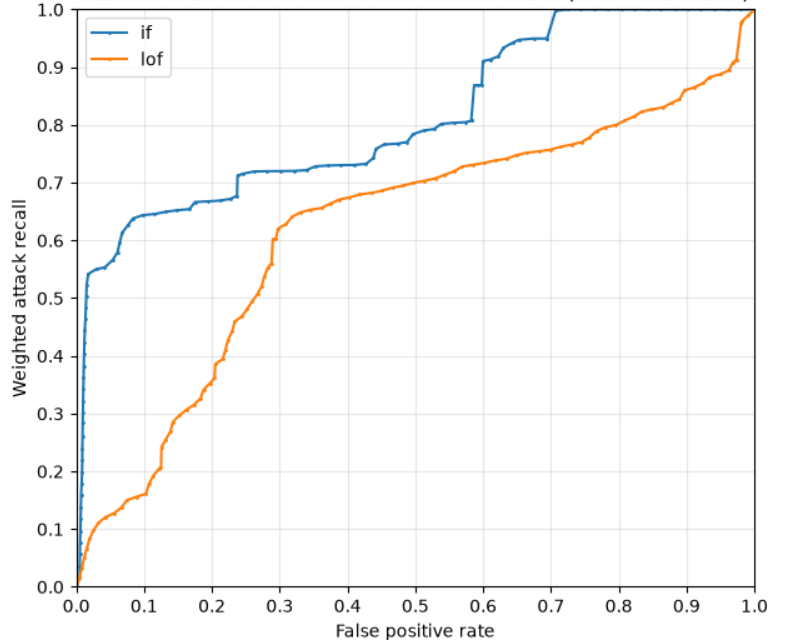
\includegraphics[width=0.8\linewidth]{Screenshot From 2026-08-26 22-59-59.png}
    \caption{Weighted attack recall vs. FPR for iForest and LOF on cross validation}
    \label{fig:placeholder}
\end{figure}
\begin{figure}[H]
    \centering
    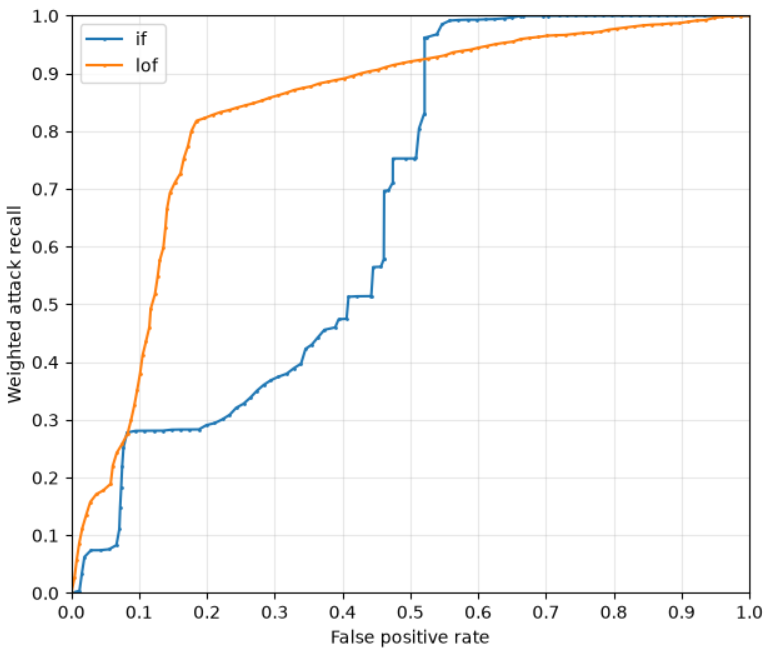
\includegraphics[width=0.8\linewidth]{Screenshot From 2026-08-26 23-03-08.png}
    \caption{Weighted attack recall vs. FPR for iForest and LOF on test}
    \label{fig:placeholder}
\end{figure}

As cross validation contains all of the anomalous flows from the training days, testing on cross-validation is also testing on unseen attacks. We can see from figure 2 that iForest always has greater attack-recall than LOF at equal FPRs. 
\par However, on the test set, LOF seems very much more proficient over the PortScan class, and beats iForest on Bot.  This is reflected by the attack-recall vs. FPR over test curves (figure 3). PortScan flows occupy 55\% of the attacks in test. Thus, LOF's ability to detect these allows it to be stronger on the test set than iForest, with much greater attack recall for the same FPR (of course, at FPRs much beyond reasonable). 
\par This contrast exposes another difficulty of zero-day detection. By definition they are unseen, unknown. Here, with unseen attacks in cross validation, I was pointed to iForest as the clearly superior model, and on test, with a new set of unseen attacks, the opposite is true. Every metric must be picked apart - individual class performance must be analysed. Specific types of attacks may be easier to be detected by certain architectures. These links must be carefully scrutinised in order for us not to become complacent. Unknown attacks may have certain fingerprints and quirks which allow them to evade detection by certain model architectures with different notions of an anomaly and different inductive biases, so in evaluation we must consider as broad a spectrum of attack classes as possible. 
\subsection{Verdict} 
While the unsupervised anomaly detection methods did greatly improve recall on unseen attack classes, they also tanked precision and caused extreme false positive rates. This is an extreme trade-off, and neither the Isolation Forest or the Local Outlier Factor methods would be deployable in a real environment. 
\section{Conclusion}
Through this project I set out to test a variety of supervised and unsupervised methods as Intrusion Detection Systems. With regards to supervised methods, the crucial finding was the collapse when introduced to unseen attacks in the test set. with all attack classes seen in training, XGBoost reaches $\sim$85\% macro attack recall, at $\sim$1-2\% FPR; with none seen, macro attack recall falls to 23\% and weighted to $\sim$1\%. Unsupervised methods partially recover novel-attack detection but at false-positive rates far too high for deployment. The difficulty with zero-day attacks persists across supervised and unsupervised methods. I implore readers to more deeply scrutinise metrics which measure only known-attack classification and ignore zero-day capability. The gap between the two is large and under-examined. 
\begin{table}[H]
\centering
\makebox[\textwidth][c]{%
\begin{tabular}{@{}llrrrrr@{}}
\toprule
\textbf{Model} & \textbf{Split}& \textbf{Test attack} & \textbf{FPR}& \textbf{Alert}& \textbf{Macro} & \textbf{Weighted} \\
& &\textbf{ classes seen} & & \textbf{precision} & \textbf{attack}& \textbf{attack}\\
& & \textbf{in training} & & & \textbf{recall} & \textbf{recall}\\
\midrule
\textbf{XGBoost (synthesis)} & Random & 14 of 14& 0.0188& 0.92& 0.85& 0.99\\ 
\textbf{XGBoost} & Temporal & 0 of 7 & 0.0115& 0.19& 0.23& 0.01 \\ 
\textbf{iForest} & Temporal & 0 of 7 & 0.0374& 0.29& 0.67& 0.46 \\ 
\textbf{LOF} & Temporal & 0 of 7 & 0.0460& 0.40& 0.76& 0.91 \\ 
\bottomrule
\end{tabular}}
\caption{Comparison of supervised and unsupervised on Random and Temporal}
\end{table}

\subsection{Limitations}
\begin{itemize}
    \item Construction issues with CIC-IDS2017 dataset. See appendix B.
    \item Due to limited compute, I took a small subsample for the Local Outlier Factor method, perhaps unfairly reducing its capability. 
    \item Greater care could have been placed on feature-scaling and hyper-parameter tuning. I took an approach that small optimisations will fundamentally be incapable of breaching the ceilings of extreme imbalance, scarcity of examples and unseen classes. However, with more time, comparisons would have been fairer in a situation where each model was fully tuned. 
    \item Only one dataset was used, thus I can not say with certainty that results about models, supervised performance or unsupervised performance, imbalance handling techniques etc. can generalise any further.
\end{itemize}
\subsection{Future Work}
In a future project or study, I could evaluate a wider range of model architectures, including reconstruction-based methods such as autoencoders. It would be valuable to see if model architecture is a valuable dial to turn for zero-day detection. However, as stated in 1.1, Moczkodan and Ragab showed the failure of many ML and DL architectures over a time-based split. They say: "architectural sophistication alone is a poor predictor of real-world IDS performance"\parencite{moczkodan2026}.
\par I could attempt to improve my results by drawing from the latest research in the ML-IDS field. Notably, the use of online / dynamic learning models which continuously update parameters when exposed to new data. Perhaps this could be an effective tool against zero-day attacks.

\begin{appendices}
\section{Networking Glossary}
\subsection{Core Concepts}
\paragraph{Packet} The basic unit of data sent over a network, containing a header (addresses, ports, flags) and a payload.
\paragraph{Flow} A sequence of packets sharing the same \textbf{5-tuple} (source IP, destination IP, source port, destination port, protocol). Each row in CIC-IDS2017 is one "conversation", rather than raw packet data. Raw network traffic must be processed into flow data to be used on models trained on the dataset.
\paragraph{Fwd and Bwd} Forwards and Backwards. Fwd = packets from initiator to responder. Bwd = Responses. Many features computed separately per direction.
\paragraph{Port} 16-bit number identifying a specific service on a host (80 is HTTP, 443 is HTTPS).
\paragraph{Protocol} Rules governing a conversation. Relevant ones include:
\begin{itemize}
  \item \textbf{TCP} - Transmission Control Protocol. Creates a link between devices with a three-way handshake (SYN, SYN-ACK, ACK). Handles ordering, error-correction and retransmission. Carries most application traffic.
  \item \textbf{UDP} - User Datagram Protocol. Fast and connectionless, sends unordered packets without asking if they arrived. Useful for DNS and streaming.
  \item \textbf{FTP} - File Transfer Protocol. Port 21. Old plaintext file-transfer service with password login.
  \item \textbf{SSH} - Secure Shell. Port 22. Encrypted remote login and command execution.
  \item \textbf{HTTP/HTTPS} - Hypertext Transfer Protocol (Secure). Port 80/443. Web traffic, unencrypted and encrypted respectively.
\end{itemize}
\paragraph{TCP flags} Single bits in TCP header signaling connection state. SYN (open), ACK (acknowledge), FIN (close politely), RST (abort), PSH (deliver now), URG (urgent).
\paragraph{IAT} Inter-Arrival Time. The gaps between consecutive packets in a flow.
\begin{table}[!htbp]
\centering
\footnotesize
\renewcommand{\arraystretch}{1.15}
\setlength{\tabcolsep}{4pt}
\begin{tabularx}{\textwidth}{@{}>{\raggedleft\arraybackslash}p{2.6cm} W{1.35} W{0.65}@{}}
\toprule
\textbf{Group} & \textbf{Examples} & \textbf{Overview} \\
\midrule
\textbf{Identifiers} & Flow ID, Source/Destination IP and Port, Protocol, \textbf{Timestamp} & Who talked to whom, when, over what service \\
\midrule 
\textbf{Duration and Counts} & Flow Duration, Total Fwd/Bwd Packets, Total Length of Fwd/Bwd Packets & Conversation size and length \\
\midrule 
\textbf{Packet length} & Fwd/Bwd Packet Length Max/Min/Mean/Std, Packet Length Variance, Average Packet Size & Shape of the payload (or lack thereof, see PortScan) \\
\midrule 
\textbf{Timing} & Flow IAT Mean/Std/Max/Min, Fwd/Bwd IAT Total and stats, Active/Idle Mean/Std/Max/Min & Rhythm of the flow \\
\midrule 
\textbf{Rates} & Flow Bytes/s, Flow Packets/s, Fwd/Bwd Packets/s & How much data is transferred per second \\
\midrule 
\textbf{Flags} & FIN/SYN/RST/PSH/ACK
/URG/CWE/ECE Flag Counts, Fwd/Bwd PSH and URG Flags & Connection behaviour and state \\
\midrule 
\textbf{Headers and TCP internals} & Fwd/Bwd Header Length, Init\_Win\_bytes\_fwd/bwd, min\_seg\_size\_forward, act\_data\_pkt\_fwd & Low-level network stack specifics. Differs between operating systems \\
\midrule 
\textbf{Bulk and subflow} & Fwd/Bwd Avg Bytes-Bulk, Packets-Bulk, Bulk Rate, Subflow Fwd/Bwd Packets and Bytes & Sustained bulk-transfer behaviour \\
\midrule 
\textbf{Ratio} & Down/Up Ratio & Asymmetry in downloads and uploads \\
\midrule 
\textbf{Target} & Label & BENIGN or attack class \\
\bottomrule
\end{tabularx}
\caption{Feature groups in CIC-IDS2017 flow representation.}
\end{table}
\subsection{CIC-IDS2017 features}
Raw packet captures were converted using the \textbf{CICFlowMeter} tool into labelled CSVs of $\sim80$ features. See table 7.

\subsection{Notes on Attack Classes}
\paragraph{Brute Force - FTP/SSH-Patator} Automated password guessing against FTP and SSH logins. Appears as many short, near-identical flows to port 21 or 22 from one source.
\paragraph{DoS (Hulk, GoldenEye, slowloris, Slowhttptest)} Single-source denial of service against a web server. Hulk and GoldenEye flood with high-volume requests. slowloris and Slowhttptest do the opposite, holding connections open with deliberately slow partial requests to exhaust the connection pool.
\paragraph{DDoS} DoS from many hosts at once, generating a large volume of concurrent flows from distinct sources. 
\paragraph{PortScan} Probing a range of ports to map open services, typically via Nmap. Produces huge numbers of tiny, short-lived flows, often with SYN sent and RST returned. 
\paragraph{Web Attack - Brute Force / XSS / SQL Injection} Attacks on a web form: credential guessing, injection scripts, injecting SQL to manipulate databases. Notably, the malicious aspects live within the payload, with minimal hints from flow statistics.
\paragraph{Infiltration} A user on the network opens a malicious file, giving an attacker a foothold, allowing them to surveil the network through the host.
\paragraph{Botnet} Hosts which are infected look to a command-and-control server for instructions. Typically features periodic, low-volume and regularly timed outbound flows.
\paragraph{Heartbleed} An OpenSSL exploit, abusing the TLS "heartbeat" to read chunks of server memory.
\section{CIC-IDS2017 Construction-Issues}
Engelen et al. (2021)\parencite{engelen2021troubleshooting} expose some severe, systemic engineering flaws in the creation of the CIC-IDS2017 dataset. Some of these flaws include issues with TCP connections terminating early, splitting single conversations into multiple flows and creating distinct tool artifacts. They also discovered many labeling errors. They produced a modified version of the dataset, reconstructing or relabeling more than 20\% of the original flows. They also identified the shortcut learning features I removed. In totality they suggest that many of the extremely high metrics ML models achieve on the dataset are due to construction issues and software bugs. With my headline statistics being model failure, not success, I see no issue in the use of the dataset for the purposes of my investigation, granted, with their feature selection and removal in place.
\end{appendices}
\printbibliography

\end{document}
